% LTeX: language=es

% En esta carpeta van los archivos que se generan al compilar el .tex (el pdf podemos moverlo a docs/ en vez de dejarlo en docs/latexFase0)
% Lo hago porque se generan como 4 o 5 archivos 

\documentclass{article}
\usepackage{graphicx} % Required for inserting images
\usepackage{underscore}
\usepackage{enumitem}
\title{Fase 0 - ICE-messAGE}
\author{Sergio Gafo Sabín \and Ander Íñiguez Bustillo \and Adrian Isábal Martín}

\begin{document}
    \pagenumbering{gobble} % Quito el número de la primera página (portada)
    \maketitle %Creo el título, especificado en la zona de preámbulo
    \newpage %Salto de página
    \pagenumbering{arabic} % Volvemos a meter los numeritos
    \section{Especificación de Requisitos}

    \subsection{Descripción general del sistema}

    El objetivo del presente proyecto es desarrollar una aplicación de mensajería que permita a los usuarios intercambiar mensajes de manera segura y confiable, haciendo uso de una arquitectura cliente/servidor con soporte P2P (Peer-to-Peer) mediante el protocolo ICE (Interactive Connectivity Establishment).\\\\
El sistema buscará establecer conexiones directas entre clientes siempre que sea posible, minimizando el uso de servidores intermedios, y permitirá que las comunicaciones continúen de forma persistente cuando los usuarios decidan almacenar sus mensajes localmente. Además, el sistema soportará la comunicación en grupos y la difusión de mensajes a canales públicos, permitiendo a múltiples usuarios participar simultáneamente en conversaciones comunes.

  \subsection{Requisitos funcionales}

El sistema deberá cumplir los siguientes requisitos funcionales:

  \begin{itemize}
    \item Permitir a un usuario identificarse de manera única mediante un nombre visible y un identificador criptográfico generado automáticamente al instalar la aplicación.
    \item Mantener una lista de usuarios activos durante la sesión, facilitando la selección de interlocutores disponibles.
    \item Establecer conexiones entre usuarios intentando primero el modo P2P y, en caso de no ser posible, recurriendo a un servidor TURN como relé de mensajes.
    \item Permitir el envío y la recepción de mensajes de texto entre usuarios.
    \item Asociar cada conversación a un identificador único derivado de las claves públicas de los participantes, de modo que se pueda continuar una conversación en sesiones posteriores si los usuarios han activado el almacenamiento.
    \item Permitir al usuario crear, unirse y gestionar grupos privados de conversación.
    \item Permitir al usuario suscribirse a canales de difusión públicos, donde varios usuarios puedan enviar y recibir mensajes simultáneamente.
    \item Permitir al usuario configurar si desea almacenar localmente el historial de conversaciones, notificando al interlocutor cuando esto esté activado.
    \item Registrar en ficheros de log las operaciones relevantes del sistema, incluyendo inicio/cierre de sesión, intentos de conexión, establecimiento de enlaces P2P o mediante TURN, envío/recepción de mensajes, y participación en grupos o canales.
    \item Proporcionar interacción con el usuario mediante dos interfaces: una por línea de comandos (CLI) y otra gráfica (GUI).
  \end{itemize}

  \subsection{Requisitos de identidad y seguridad}

  \begin{itemize}
    \item Cada cliente generará un par de claves criptográficas (privada y pública) al instalar la aplicación. La clave pública servirá como identificador único del usuario.
    \item Las conversaciones se identificarán mediante un hash derivado de las claves públicas de los participantes, garantizando que los mensajes se asocien correctamente en sesiones posteriores.
    \item Todas las comunicaciones estarán cifradas mediante protocolos seguros (DTLS/TLS), tanto en conexiones P2P como cuando se utilice el servidor TURN.
    \item La participación en grupos y canales respetará los mismos mecanismos de identidad y autenticación, asegurando que cada mensaje pueda atribuirse correctamente a un usuario único.
  \end{itemize}

  \section{Arquitectura del Sistema}
    El sistema de comunicaciones de la aplicación es una implementación del protocolo ICE (Interactive Connectivity Establishment, RFC 8445) para intentar establecer una conexión P2P siempre que sea posible para evitar al máximo las conexiones por servidor, pero que también usuarios tras una red NAT simétrica (que imposibilita las conexiones P2P) puedan utilizar la aplicación. Este protocolo cuenta con varios componentes principales además de la aplicación cliente:
    
    \subsection{Componentes}
    \subsubsection{Servidor tracker}
    Actúa como punto de encuentro entre peers. Su función solo es de control: gestiona las conexiones de los clientes, mantiene un registro de usuarios activos y retransmite los mensajes de señalización entre ellos. Es decir, su único objetivo es establecer una conexión entre dos clientes que lo soliciten. \vspace{1em}
    
    Protocolos:
    
    \begin{itemize}
       \item Capa de transporte: TCP
       \item Capa de aplicación: WebSockets
       \item Capa de seguridad: TLS
    \end{itemize}

    
    \subsubsection{Servidor STUN}
    Servidor auxiliar que permite a un cliente descubrir su dirección y puerto públicos tal como son vistos desde Internet. Esta información es necesaria para que otros peers puedan intentar conectarse con él. \vspace{1em}
    
    Protocolos:
    
    \begin{itemize}
       \item Capa de transporte: UDP
       \item Capa de aplicación: STUN
       \item Capa de seguridad: DTLS
    \end{itemize}
    
    \subsubsection{Servidor TURN}
    Server de retransmisión de los datos para cuando las conexiones P2P son imposibles por topología de alguna de las redes de los host. El cliente reserva una dirección y puerto en el servidor TURN, y todos los mensajes cifrados se envían a este servidor, que los reenvía al otro peer. \vspace{1em}
    
    Protocolos:
    
    \begin{itemize}
       \item Capa de transporte: TCP
       \item Capa de aplicación: TURN
       \item Capa de seguridad: TLS
    \end{itemize}
    
    \subsubsection{Host de P2P}
    En los casos en los que sea posible (cosa que cada dispositivo identificará primero verificando con el servidor STUN si se encuentra en una red que admita conexiones P2P, y después verificando si el peer con el que se quiere conectar también admite este tipo de conexiones y tiene dirección IP:puerto obtenibles via tracker) los clientes intercambiarán mensajes vía conexiones P2P. Estas conexiones funcionarán mediante: \vspace{1em}
    
    Protocolos:
    
    \begin{itemize}
       \item Capa de transporte: UDP
       \item Capa de aplicación: SCTP
       \item Capa de seguridad: DTLS
    \end{itemize}

    \section{Interfaz de Usuario}

    \begin{center}
    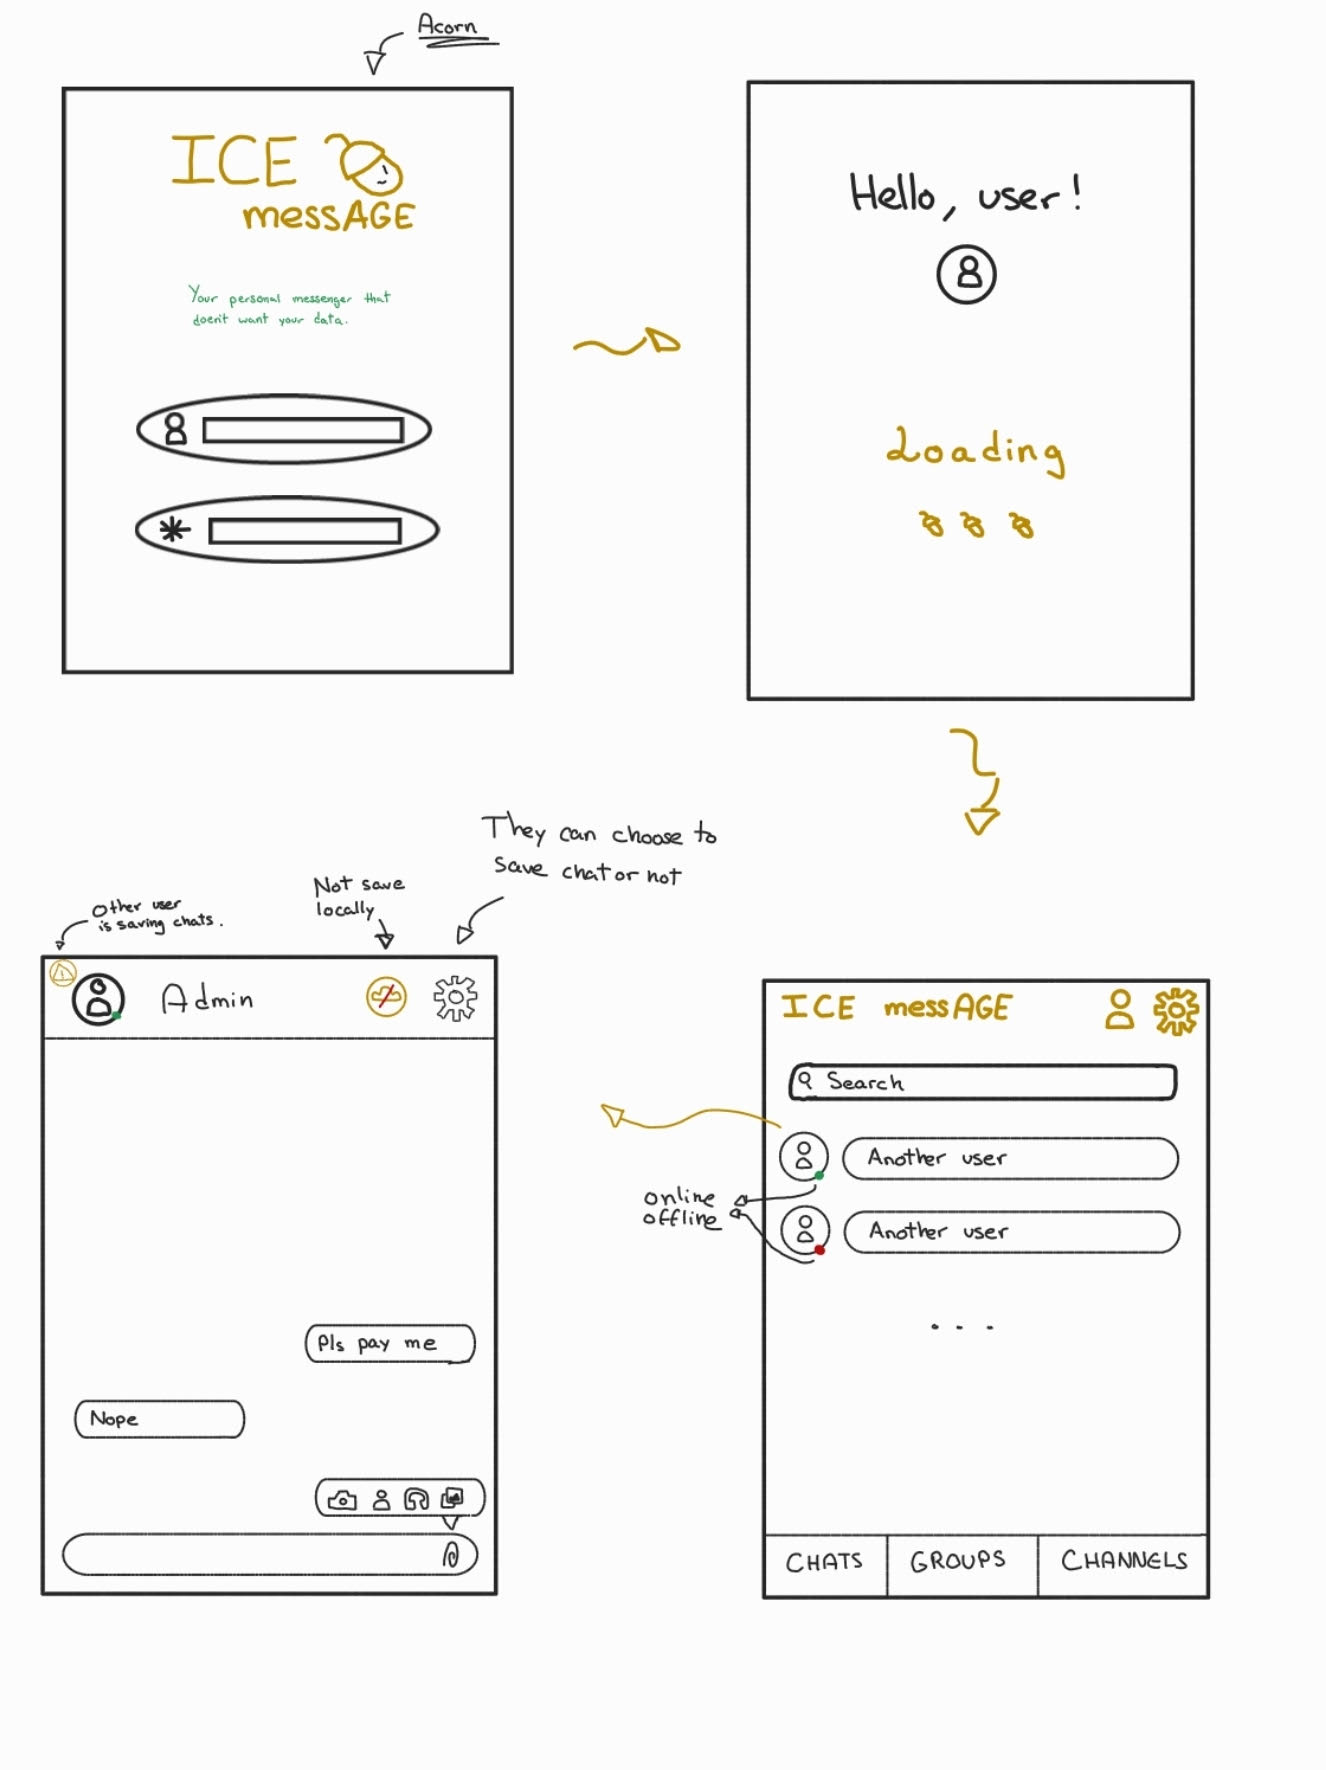
\includegraphics[width=1.2\linewidth]{diseÑo.jpg}
    \end{center}

    \section{Estructura de Ficheros}

  \begin{verbatim}

/ICE-messAGE/
|
|-- src/                     # Código fuente
|   |-- main.c 
|   |-- cli/                 # Implementación CLI (.c / .cpp / .h)
|   |-- gui/                 # Implementación GUI (.cpp / .h)
|   |-- core/                # Funciones principales y cifrado (.c / .cpp / .h)
|   |-- network/             # Tracker, STUN, TURN, P2P (.c / .cpp / .h)
|   \-- utils/               # Funciones auxiliares (.c / .cpp / .h)
|
|-- include/                 # Archivos de cabecera compartidos (.h / .hpp)
|
|-- build/                   # Archivos de compilación temporales
|   \-- ...
|
|-- config/                  # Archivos de configuración
|   |-- server.config          
|   \-- client.config         
|
|-- data/                    # Datos persistentes del usuario
|   \-- database.db          # Claves públicas, historial opcional
|
|-- logs/                    # Registros operaciones
|   \-- app.log
|
\-- scripts/                
    \-- Makefile

  \end{verbatim}

La estructura de ficheros del proyecto está organizada para mantener claridad y modularidad. La carpeta src/ contiene todo el código fuente, con un archivo main que inicia la aplicación y llama a los módulos de la interfaz correspondiente (cli/ o gui/). Los módulos core/, network/ y utils/ contienen el funcionamiento principal de la aplicación, la conexión P2P y las funciones auxiliares, mientras que include/ almacena los archivos de cabecera compartidos. La configuración, los datos del usuario y los registros se encuentran en config/, data/ y logs/, por otro lado, scripts/ contiene los archivos necesarios para compilar y ejecutar el proyecto. Esta organización permite entender rápidamente cómo está estructurado el proyecto y facilita trabajar en distintas partes del código sin confusión.

\section{Esquemas de la BBDD}

 \begin{center}
 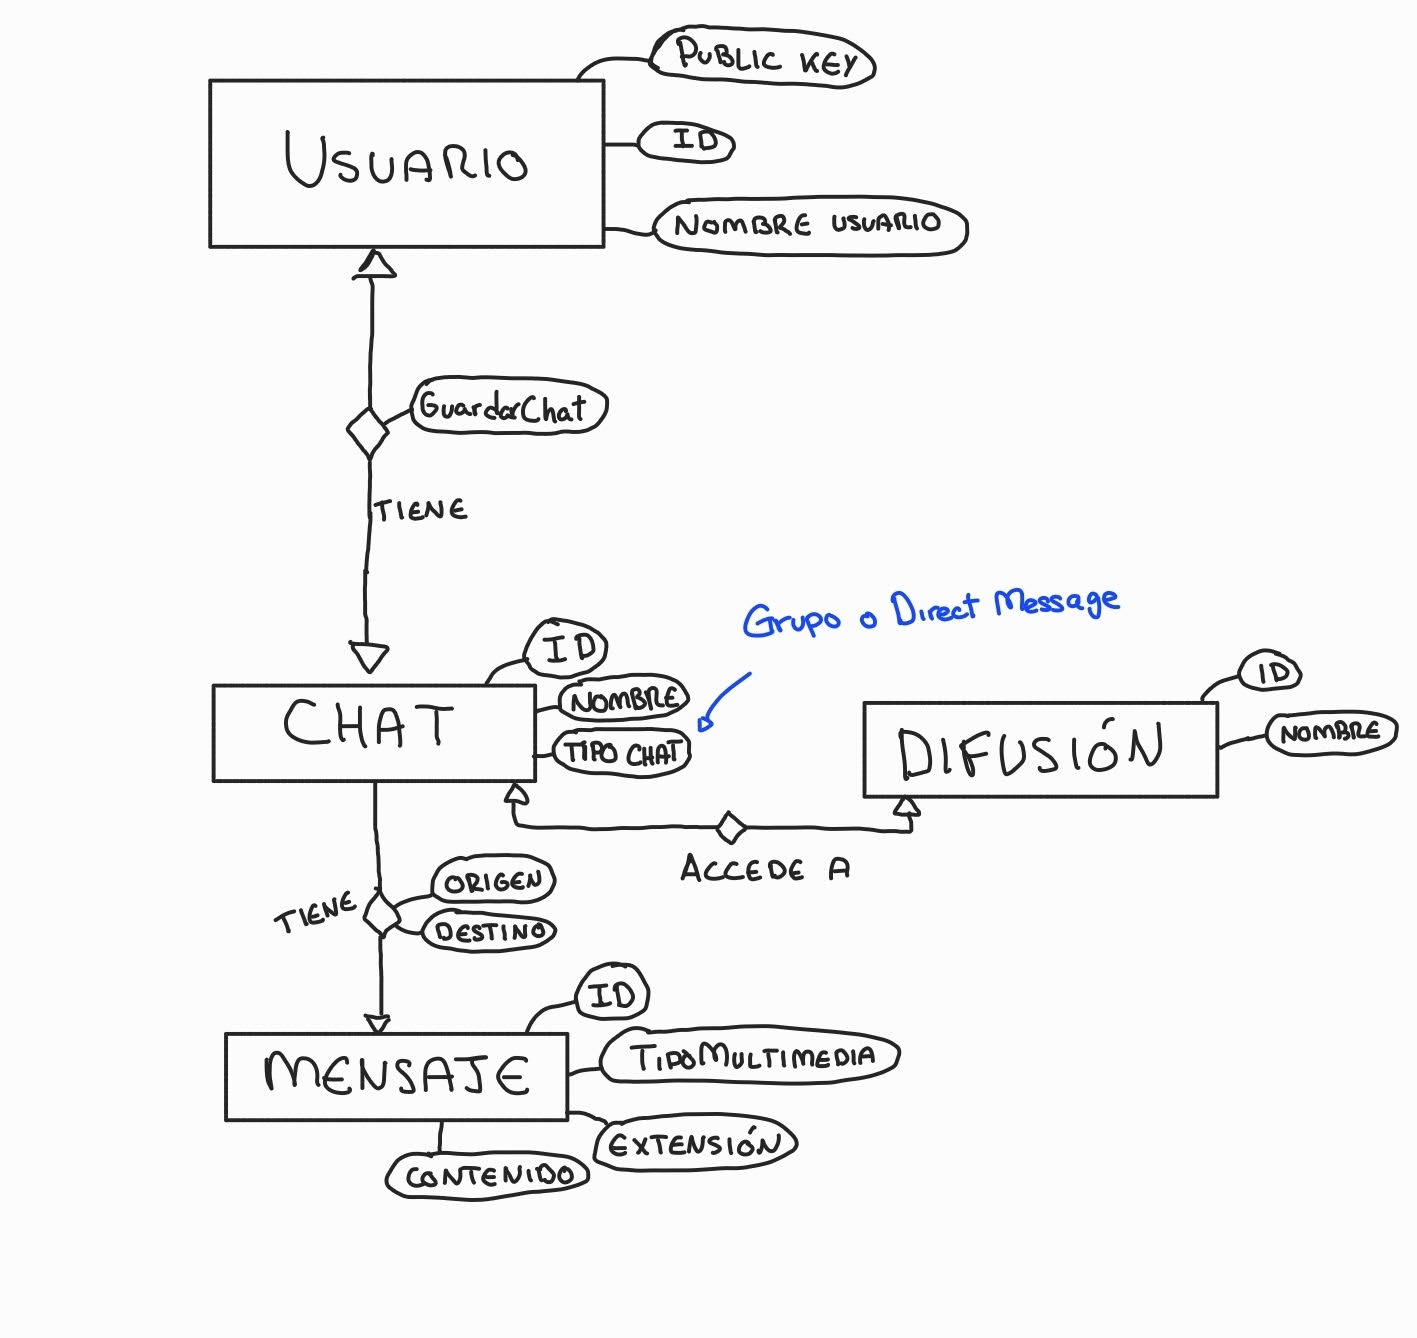
\includegraphics[width=1.2\linewidth]{bbdd.jpg}
 \end{center}

\section{Protocolo de comunicaciones}
    \subsection{Ejemplo de diálogo completo}
    
    El flujo de una posible interacción entre los clientes A y B y el tracker T, el servidor STUN S y el servidor TURN R actuando como intermediarios:

    \subsubsection{Parte fija}

    \begin{enumerate}
        \item A y B envían una petición a S para descubrir su IP:puerto público y topología de red (para saber de antemano si las conexiones P2P son posibles)
        \item A y B se conectan a T mediante WebSockets seguros (WSS) y envía un mensaje de registro que incluye: nombre de usuario, dirección pública descubierta, tipo de NAT y clave pública de cifrado.
        \item Cliente A solicita iniciar conversación con B enviando un mensaje call_request al tracker.
        \item El tracker reenvía la petición a Cliente B. Este acepta y responde con un call_response (accepted=true) a través del tracker, que llega a A.
    \end{enumerate}
    
    \textbf{Conexión P2P:}
    \begin{enumerate}[label=\arabic*., start=6]
        \item A y B realizan hole punching sincronizados mediante el servidor STUN.
        \item En caso exitoso, negocian DTLS y establecen un stream SCTP por el que podrán enviarse los mensajes.
    \end{enumerate}

    \textbf{Conexión por relay:}
    \begin{enumerate}[label=\arabic*., start=6]
        \item Hole punching falla o se descarta si las topologías de red notificadas al tracker no lo permiten
        \item A y B envian allocate a R para obtener direcciones relay que se notifican mutuamente a través de T
        \item A y B establecen conexión TCP con R, negocian TLS y pueden intercambiar mensajes cifrados hasta que cierren la conexión
    \end{enumerate}

    \subsection{Formato de los mensajes}
    \begin{itemize}
        \item Comunicaciones con STUN: RFC 8489
        \item Comunicaciones con TURN: RFC 8656
        \item Envío de datos P2P: RFC 8832 (Data Channel Establishment)
        \item Comunicaciones por tracker: Protocolo propio
            \begin{itemize}
                \item Tipo de mensaje: 1 byte (0x01 = register, 0x02 = call_request, 0x03 = ice_candidate, etc.)
                \item Flags (1 byte): indicadores de control
                \item ID de transacción (4-8 bytes): para correlacionar respuestas
                \item Payload (datos de usuario (clave pública, puerto, etc))
            \end{itemize}
    \end{itemize}
\end{document}
    
